\chapter{Estado de la cuestión}
\label{chap:estado_cuestion}

En la actualidad, la generación de música o, en un sentido ámplio, de sonido, constituye uno de los frentes de investigación activos y más prometedores en el campo de la IA. La generación música con modelos de \textit{Deep Learning} ha sido abordado históricamente desde dos grandes perspectivas en función de la naturaleza de los datos generados por los modelos: la generación de música simbólica y la generación de música con audio. La primera de ellas consiste en la creación de elementos musicales como notas, acordes, melodías, etc. en un formato simbólico, ya sea MIDI, OSC, MusicXML, ABC, Lilypond, o cualquier formato musical reducible a símbolos textuales. La segunda, en la creación de archivos de audio directamente reproducibles. 

...Seguir para esta sección el estado de la cuestión que se ofrece en \cite{hernandez-olivanSurveyArtificialIntelligence2022}, que es muy completo. 
Tras esto, exponer los modelos actuales de generación de audio.
Mostrar que nuestro trabajo se focaliza en la generación de música simbólica pero restringida a la generación de código de programación sonora con LLM no entrenados específicamente para ello.
 


\begin{itemize}
    \item Modelos de IA generativa aplicados a la música.
    \item LLM asistentes para la creación de código de programación.
    \item Lenguajes de programación musical.
    \item Prompting engineering.
    \item LLM y música (MIDI y otras representaciones).
    \item LLM y música con lenguajes de programación.
\end{itemize}

\section{Modelos de IA generativa aplicados a la música}
    Repasar especialmente los últimos modelos lanzados por Google y Amazon\dots y su estado.

\section{LLM asistentes para la creación de código de programación}
\label{sec:llm_asistentes_creacion_codigo_programacion}
    GPT-4 como estado del arte. Software específico como Github Copilot. Hablar de los más importantes LLM y su rendimiento en la programación.


    \begin{figure}[h]
        \caption{Relación AI, ML y DL}
        \centering
        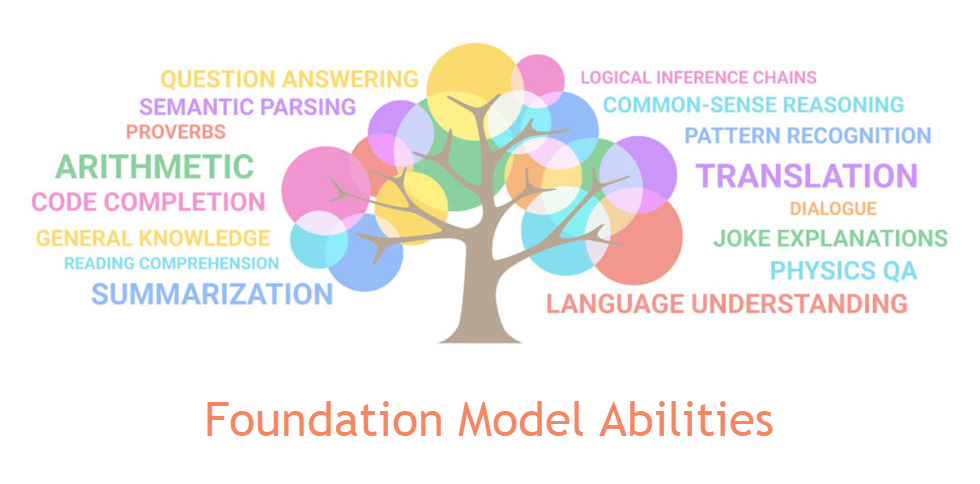
\includegraphics[width=0.8\textwidth]{./figuras/fundation_models_habilities.png}
        \source{\cite{GPT3RiseFoundation}}
        \label{fig:fundation_models_habilities}
    \end{figure}

\section{Lenguajes de programación musical}
    Lenguajes a modo de código de programación, como Overtone, Pure Data, Sonic Pi, Supercollider, Max MSP. Representaciones musicales susceptibles de ser generadas por LLM, como el MIDI, MusicXML, ABC, Lilypond, etc.

\section{Prompting engineering. Estado del arte}
    Un repaso por los papers más significativos y actuales sobre esta cuestión, especialmente las que implican la generación de código.

\section{\textit{Retrieval-Augmented Generation} (RAG)}
    Una de las técnicas más potentes para la generación de código, que combina la recuperación de información con la generación de texto. También de OpenAI Assistant, que ha presentado en el Keynote de 2023. \cite{WhatRetrievalaugmentedGeneration2021} y \cite{lewisRetrievalAugmentedGenerationKnowledgeIntensive2021}

\section{LLM y música (MIDI y otras representaciones) y el problema del significado}
    Quiero exponer la distancia que supone conocer un lenguaje y usarlo para crear arte con él. Que un sistema (o un ser humano) conozca la sintaxis de un lenguaje no significa que pueda crear con él obras de arte... al menos si no se le entrena con suficientes datos.
    
    Usar como bibliografía: el paper \cite{lewisRetrievalAugmentedGenerationKnowledgeIntensive2021} y la web \cite{WhatRetrievalaugmentedGeneration2021}

\section{LLM y música en SuperCollider}